\documentclass[tikz,border=2pt]{standalone}
\usepackage{amsmath}
\usetikzlibrary{arrows.meta}
\begin{document}
% Entry with an unknown type: Nature draws C (prob p) or W (1-p); the entrant (blue) sees its type and
% chooses Out (entrant gets 0) or In; the incumbent (red) sees only In, so its two nodes form one
% information set with belief mu on C. Fight pays the incumbent 2 - 3 mu, Accommodate 1, so Fight
% iff mu <= 1/3. Thick green: the pooling PBE for p = 1/2 (both types In, mu = 1/2, Accommodate).
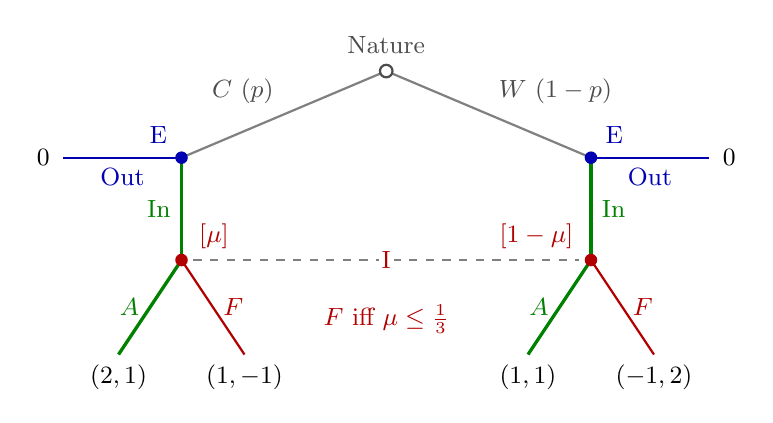
\begin{tikzpicture}[font=\small, >={Latex[length=2mm]},
    dec/.style={circle, fill, inner sep=1.6pt}]
  % Nature
  \draw[thick, gray] (0,0) -- node[above left, gray!60!black] {$C$ $(p)$} (-2.6,-1.1);
  \draw[thick, gray] (0,0) -- node[above right, gray!60!black] {$W$ $(1-p)$} (2.6,-1.1);
  \node[circle, draw, thick, gray!60!black, fill=white, inner sep=1.6pt, label={[gray!60!black]above:Nature}] at (0,0) {};
  % entrant: Out
  \draw[thick, blue!70!black] (-2.6,-1.1) -- node[below] {Out} (-4.1,-1.1);
  \draw[thick, blue!70!black] (2.6,-1.1) -- node[below] {Out} (4.1,-1.1);
  \node[anchor=east] at (-4.15,-1.1) {$0$};
  \node[anchor=west] at (4.15,-1.1) {$0$};
  % entrant: In (on the pooling path)
  \draw[very thick, green!50!black] (-2.6,-1.1) -- node[left] {In} (-2.6,-2.4);
  \draw[very thick, green!50!black] (2.6,-1.1) -- node[right] {In} (2.6,-2.4);
  \node[dec, blue!70!black, label={[blue!70!black]above left:E}] at (-2.6,-1.1) {};
  \node[dec, blue!70!black, label={[blue!70!black]above right:E}] at (2.6,-1.1) {};
  % incumbent
  \draw[very thick, green!50!black] (-2.6,-2.4) -- node[left] {$A$} (-3.4,-3.6);
  \draw[thick, red!70!black] (-2.6,-2.4) -- node[right] {$F$} (-1.8,-3.6);
  \draw[very thick, green!50!black] (2.6,-2.4) -- node[left] {$A$} (1.8,-3.6);
  \draw[thick, red!70!black] (2.6,-2.4) -- node[right] {$F$} (3.4,-3.6);
  \draw[dashed, thick, gray] (-2.45,-2.4) -- (2.45,-2.4);
  \node[dec, red!70!black] at (-2.6,-2.4) {};
  \node[dec, red!70!black] at (2.6,-2.4) {};
  \node[red!70!black, anchor=south west] at (-2.5,-2.38) {$[\mu]$};
  \node[red!70!black, anchor=south east] at (2.5,-2.38) {$[1-\mu]$};
  \node[red!70!black, fill=white, inner sep=1pt] at (0,-2.4) {I};
  \node[red!70!black] at (0,-3.15) {$F$ iff $\mu\le\tfrac13$};
  % payoffs (entrant, incumbent)
  \foreach \x/\p in {-3.4/{(2,1)}, -1.8/{(1,-1)}, 1.8/{(1,1)}, 3.4/{(-1,2)}}
    \node[anchor=north, inner sep=2pt] at (\x,-3.65) {$\p$};
\end{tikzpicture}
\end{document}
